\documentclass[12pt]{article}
\usepackage{amsfonts,amssymb,float,amsmath}
\usepackage{algorithmic}
\usepackage{graphicx, siunintx}
\usepackage{textcomp}
\usepackage{xcolor}
\usepackage{txfonts}
\usepackage{multicol}
\usepackage{listings}
\usepackage{enumitem}
\usepackage{mathtools}
\usepackage{gensymb}
\usepackage{comment}
\usepackage[breaklinks=true]{hyperref}
\usepackage{tkz-euclide} 
\usepackage{listings}
\usepackage{gvv}                       
\usepackage{gvv-book}
%\def\inputGnumericTable{}                             
\usepackage{color}                                            
\usepackage{array}                                            
\usepackage{longtable}                                       
\usepackage{calc}                                             
\usepackage{multirow}                                         
\usepackage{hhline}                                           
\usepackage{ifthen}                                           
\usepackage{lscape}
\newcommand{\BEQA}{\begin{eqnarray}}
\newcommand{\EEQA}{\end{eqnarray}}
%\newcommand{\define}{\stackrel{\triangle}{=}}
\theoremstyle{remark}
\newtheorem{rem}{Remark}
\parindent 0px
\pagenumbering{gobble}
\begin{document}
\title{\vspace{-5cm}Gate paper 2023-XH}
\author{Ayush Sunil Labhade}
\date{AI25Btech11002}
\maketitle
\begin{flushright}Humanities and Social Sciences-Economics\end{flushright}
\begin{flushleft}General Aptitude \textbf{\brak{GA}} \\[5pt]
\textbf{\item Q.1 - Q.5 Carry ONE mark each}\end{flushleft}
%Q.1
\begin{enumerate}
\item Rafi told Mary, “I am thinking of watching a film this weekend.”
The following reports the above statement in indirect speech:
Rafi told Mary that he $\_\_\_\_\_\_$ of watching a film that weekend. 
\begin{enumerate} \begin{multicols}{2}
\item  thought
\item  is thinking 
\item  am thinking
\item  was thinking 
\end{multicols} \end{enumerate}
\hfill\brak{GATE \ XH \ 2025}
%Q.2
\item Permit : $\_\_\_\_\_\_$ :: Enforce : Relax
\brak{By\ word\ meaning}\newline
\begin{enumerate} \begin{multicols}{4} 
\item Allow 
\item Forbid 
\item License
\item Reinforce
\end{multicols} \end{enumerate}
\hfill\brak{GATE \ XH \ 2025}
%Q.3
\item Given a fair six-faced dice where the faces are labelled ‘1’, ‘2’, ‘3’, ‘4’, ‘5’, and ‘6’, what is the probability of getting a ‘1’ on the first roll of the dice and a ‘4’ on the second roll?
\begin{enumerate} \begin{multicols}{4}
\item $\frac{1}{36}$
\item $\frac{1}{6}$
\item $\frac{5}{6}$
\item $\frac{1}{3}$ 
\end{multicols} \end{enumerate}
\hfill\brak{GATE \ XH \ 2025}
%Q.4
\item A recent survey shows that 65\% of tobacco users were advised to stop consuming tobacco. The survey also shows that 3 out of 10 tobacco users attempted to stop using tobacco.\\
Based only on the information in the above passage, which one of the following options can be logically inferred with \textit{certainty}?
\begin{enumerate}
\item A majority of tobacco users who were advised to stop consuming tobacco made an attempt to do so.
\item A majority of tobacco users who were advised to stop consuming tobacco did not attempt to do so. 
\item Approximately 30\% of tobacco users successfully stopped consuming tobacco. 
\item Approximately 65\% of tobacco users successfully stopped consuming tobacco.
\end{enumerate}
\hfill\brak{GATE \ XH \ 2025}
\newline
%Q.5
\item How many triangles are present in the given figure
\begin{centering}
\begin{figure}[H] 
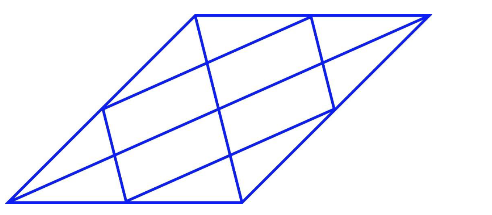
\includegraphics{Figs/Q5.png}
\caption{}
\label{Fig:1.1} 
\end{figure}
\end{centering}
\begin{enumerate} \begin{multicols}{4}
\item 12
\item 16 
\item 20 
\item 24 
\end{multicols} \end{enumerate}
\hfill\brak{GATE \ XH \ 2025}
\newpage
\textbf{Q.6- Q.10 Carry TWO marks Each} 
%Q.6
\item Students of all the departments of a college who have successfully completed the registration process are eligible to vote in the upcoming college elections. However, by the time the due date for registration was over, it was found that surprisingly none of the students from the Department of Human Sciences had completed the registration process.Based only on the information provided above, which one of the following sets of statement(s) can be logically inferred with certainty?
\begin{enumerate}
\item [(i)] All those students who would not be eligible to vote in the college elections would certainly belong to the Department of Human Sciences.
\item [(ii)] None of the students from departments other than Human Sciences failed to complete the registration process within the due time.
\item [(iii)] All the eligible voters would certainly be students who are not from the Department of Human Sciences.
\end{enumerate} 
\begin{enumerate} \begin{multicols}{4}
\item (i) and (ii) 
\item (i) and (iii) 
\item only (i)
\item only (iii) 
\end{multicols} \end{enumerate}
\hfill\brak{GATE \ XH \ 2025}
%Q.7
\item  Which one of the following options represents the given graph? 
\begin{figure}[H]
\centering
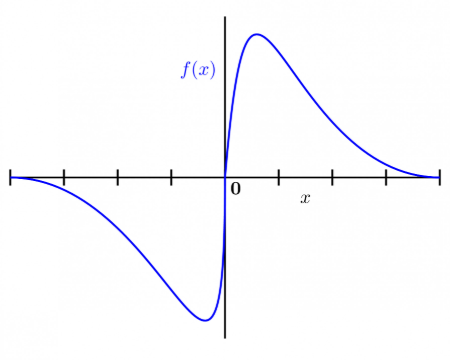
\includegraphics{Figs/Q7.png}
\caption{}
\label{Fig:1.2}
\end{figure}
\begin{enumerate} \begin{multicols}{4}
\item $f(x)=x^22^{-|x|}$ 
\item $f(x)=x2^{-|x|}$
\item $f(x)=|x|2^{-x}$ 
\item $f(x)=x2^{-x}$
\end{multicols} \end{enumerate}
\hfill\brak{GATE \ XH \ 2025}
%Q.8
\item Which one of the options does NOT describe the passage below or follow from it? 
 We tend to think of cancer as a ‘modern’ illness because its metaphors are so modern. It is a disease of overproduction, of sudden growth, a growth that is unstoppable, tipped into the abyss of no control. Modern cell biology encourages us to imagine the cell as a molecular machine. Cancer is that machine unable to quench its initial command (to grow) and thus transform into an indestructible, self-propelled automaton.\\
\sbrak{Adapted from \textit{The Emperor of All Maladies} by Siddhartha Mukherjee}
\begin{enumerate}
\item   It is a reflection of why cancer seems so modern to most of us. 
\item   It tells us that modern cell biology uses and promotes metaphors of machinery. 
\item   Modern cell biology encourages metaphors of machinery, and cancer is often imagined as a machine. 
\item   Modern cell biology never uses figurative language, such as metaphors, to describe or explain anything. 
\end{enumerate}
\hfill\brak{GATE \ XH \ 2025}
%Q.9
\item The digit in the unit’s place of the product $3^{999} \times 7^{1000}$ is \\ 
\begin{enumerate} \begin{multicols}{2}
\item   7 
\item   1  
\item   4  
\item   9 
\end{multicols} \end{enumerate}
\hfill\brak{GATE \ XH \ 2025}
%Q.10
\item A square with sides of length 6 cm is given. The boundary of the shaded region is defined by two semi-circles whose diameters are the sides of the square, as shown. The area of the shaded region is \_\_\_\_ cm$^2$
\begin{figure}[H]
\centering
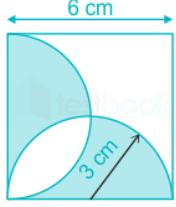
\includegraphics{Figs/Q10.png}
\caption{}
\label{Fig:1.3}
\end{figure} 
\begin{enumerate} \begin{multicols}{4} 
\item   $6\pi$
\item   18 
\item   20 
\item   $9\pi$ 
\end{multicols} \end{enumerate}
\hfill\brak{GATE \ XH \ 2025}
\newpage
\textbf{Reasoning and Comprehension(XH-B1)\newline 
XH-B1:Q11-Q17 Carry ONE mark Each}
%Q.11
\item  Which word below best describes the idea of being both \textit{Spineless} and \textit{Cowardly}? 
\begin{enumerate} \begin{multicols}{4}
\item   Pusillanimous 
\item   Unctuous 
\item   Obsequious 
\item   Reticent  

\end{multicols} \end{enumerate}
\hfill\brak{GATE \ XH \ 2025}
%Q.12
\item   Choose the right preposition to fill up the blank: \newline
 The whole family got together \_\_ Diwali  
 \begin{enumerate} \begin{multicols}{4}
\item   of 
\item   at 
\item   in  
\item   till  

\end{multicols} \end{enumerate}
\hfill\brak{GATE \ XH \ 2025}
%Q.13
\item  Select the correct option to fill in all the blanks to complete the passage:

The (i) \_\_\_\_\_\_\_\_\_ factor amid this turbulence has been the (ii) \_\_\_\_\_\_\_\_\_ of high-octane, action-oriented films such as RRR, K.G.F: Chapter 2 and Pushpa from film industries in the south of the country. Traditionally, films made in the south have done well in their own (iii) \_\_\_\_\_\_\_\_\_. But increasingly, their dubbed versions have performed well in the Hindi heartland, with collections (iv) \_\_\_\_\_\_\_\_\_ those of their Bollywood counterparts. \\
\begin{enumerate} 
\item   (i) disheartening \quad (ii) failure \quad (iii) channels \quad (iv) matching 
\item   (i) redeeming \quad (ii) outperformance \quad (iii) geographies \quad (iv) eclipsing 
\item   (i) shocking \quad (ii) underperformance \quad (iii) cinemas \quad (iv) below 
\item   (i) humbling \quad (ii) bombing \quad (iii) theatres \quad (iv) falling behind 
 \end{enumerate}
\hfill\brak{GATE \ XH \ 2025}
%Q.14
\item  The following passage consists of 6 sentences.
The first and sixth sentences of the passage are at their correct positions, while the middle four sentences (represented by 2, 3, 4, and 5) are jumbled up.
Choose the correct sequence of the sentences so that they form a coherent paragraph:
\begin{enumerate}
\item  Most obviously, mobility is taken to be a geographical as well as a social phenomenon.
\item  Much of the social mobility literature regarded society as a uniform surface and failed to register the geographical intersections of region, city and place, with the social categories of class, gender and ethnicity.
\item  The existing sociology of migration is incidentally far too limited in its concerns to be very useful here.
\item  Further, I am concerned with the flows of people within, but especially beyond, the territory of each society, and how these flows may relate to many different desires, for work, housing, leisure, religion, family relationships, criminal gain, asylum seeking and so on.
\item  Moreover, not only people are mobile but so too are many ‘objects’.
\item  I show that sociology’s recent development of a ‘sociology of objects’ needs to be taken further and that the diverse flows of objects across societal borders and their intersections with the multiple flows of people are hugely significant. 
\end{enumerate}
\begin{enumerate} \begin{multicols}{4}
\item   3,2,5,4 
\item   2,3,4,5 
\item   5,4,3,2 
\item   4,2,5,3 
\end{multicols} \end{enumerate}
\hfill\brak{GATE \ XH \ 2025}
%Q.15
\item The population of a country increased by 5\% from 2020 to 2021. Then, the population decreased by 5\% from 2021 to 2022. By what percentage did the population change from 2020 to 2022? 
\begin{enumerate} \begin{multicols}{4}
\item   -0.25\% 
\item   0\% 
\item   2.5\% 
\item   10.25\% 
\end{multicols} \end{enumerate}
\hfill\brak{GATE \ XH \ 2025}
%Q.16
\item The words \textbf{Thin: Slim: Slender} are related in some way. Identify the correct option(s) that reflect(s) the same relationship: 
\begin{enumerate} \begin{multicols}{2}
\item   Fat: Plump: Voluptuous 
\item   Short: Small: Petite 
\item   Tall: Taller: Tallest 
\item   Fair: Dark: Wheatish 
\end{multicols} \end{enumerate}
\hfill\brak{GATE \ XH \ 2025}
%Q.17
\item  A pandemic like situation hit the country last year, resulting in loss of human life and economic depression. To improve the condition of its citizens, the government made a series of emergency medical interventions and increased spending to revive the economy. In both these efforts, district administration authorities were actively involved.
Which of the following action(s) are plausible? \\
\begin{enumerate}
\item   In future, the government can make district administration authorities responsible for protecting health of citizens and reviving the economy. 
\item   The government may set up a task force to review the post pandemic situation and ascertain the effectiveness of the measures taken. 
\item   The government may set up a committee to formulate a pandemic management program to minimize losses to life and economy in future.
\item   The government may take population control measures to minimize pandemic related losses in future. 
\end{enumerate}
\hfill\brak{GATE \ XH \ 2025}
\newpage
\textbf{XH-B1:Q18-Q26 Carry TWO mark Each}
%Q.18
\item Six students, Arif, Balwinder, Chintu, David, Emon and Fulmoni appeared in the GATE-XH exam in 2022. Balwinder scores less than Chintu in XH-B1, but more than Arif in XH-C1. David scores more than Balwinder in XH-C1, and more than Chintu in XH-B1. Emon scores less than David, but more than Fulmoni in XH-B1. Fulmoni scores more than David in XH-C1. Arif scores less than Emon, but more than Fulmoni in XH-B1. Who scores highest in XH-B1? 
\begin{enumerate} \begin{multicols}{4}
\item   Fulmoni 
\item   Emon 
\item   David 
\item   Chintu 
\end{multicols} \end{enumerate}
\hfill\brak{GATE \ XH \ 2025}
%Q.19
\item Select the correct relation between E and F.
$$
E = \frac{x}{1 + x} \quad \text{and} \quad F = \frac{-x}{1 - x} \quad x > 1
$$ 
\begin{enumerate} \begin{multicols}{4}
\item   $E > F$ 
\item   $E < F$ 
\item   $E = F$ 
\item   $E < -F$ 
\end{multicols} \end{enumerate}
\hfill\brak{GATE \ XH \ 2025}
%Q.20
\item  A code language is formulated thus:
\vspace{1mm}
Vowels in the original word are replaced by the next vowel from the list of vowels, A-E-I-O-U (For example, E is replaced by I and U is replaced by A). Consonants in the original word are replaced by previous consonant (For example, T is replaced by S and V is replaced by T).
\vspace{1mm}
Then how does the word, GOODMORNING appear in the coded language? 
\begin{enumerate} \begin{multicols}{2}
\item   HUUFNUSPOPH 
\item   FIICLIQMEMF 
\item   FUUCLIUQMOMF 
\item   HEEDATTACRH 
\end{multicols} \end{enumerate}

\hfill\brak{GATE \ XH \ 2025}
%Q.21
\item  The stranger is by nature no "owner of soil" -- soil not only in the physical, but also in the figurative sense of a life-substance, which is fixed, if not in a point in space, at least in an ideal point of the social environment. Although in more intimate relations, he may develop all kinds of charm and significance, as long as he is considered a stranger in the eyes of the other, he is not an "owner of soil." 
\newline
Restriction to intermediary trade, and often (as though sublimated from it) to pure finance, gives him the specific character of mobility. If mobility takes place within a closed group, it embodies that synthesis of nearness and distance which constitutes the formal position of the stranger. For, the fundamentally mobile person comes in contact, at one time or another, with every individual, but is not organically connected, through established ties of kinship, locality, and occupation, with any single one.
\vspace{1mm}
What assumptions can be made about the stranger from the passage above? \\
\begin{enumerate} 
\item   The stranger can become an owner of soil through developing all kinds of charm in more intimate relations. 
\item   The stranger cannot become an owner of soil either in the physical or psychological sense. 
\item   The stranger can become an owner of soil through establishing ties of kinship and so on.
\item   The stranger might become an owner of soil in the physical sense but not in the psychological. 
\end{enumerate}
\hfill\brak{GATE \ XH \ 2025}
%Q.22
\item L is the only son of A and S. S has one sibling, B, who is married to L’s aunt, K. B is the only son of D. How are L and D related?
\vspace{1mm}

Select the possible option(s):\\ 
\begin{enumerate} 
\item   Grandchild and Paternal Grandfather 
\item   Grandchild and Maternal Grandfather 
\item   Grandchild and Paternal Grandmother 
\item   Grandchild and Maternal Grandmother 
\end{enumerate}
\hfill\brak{GATE \ XH \ 2025}
%Q.23
\item Five segments of a sentence are given below. The first and fifth segments are at their correct positions, while the middle three segments (represented by 2, 3, and 4) are jumbled up. Choose the correct order of the segments so that they form a coherent sentence:
\begin{enumerate} 
\item[1.]  Consumed multitudes are jostling and shoving inside me
\item[2.]  and guided only by the memory of a large white bedsheet with a roughly circular hole some seven inches in diameter cut into the center,
\item[3.]  clutching at the dream of that holey, mutilated square of linen, which is my talisman, my open-sesame, 
\item[4.]  I must commence the business of remaking my life from the point at which it really began,
\item[5.]  some thirty-two years before anything as obvious, as present, as my clock-ridden, crime-stained birth
\end{enumerate}
\begin{enumerate} \begin{multicols}{4}
\item   2-3-4 
\item  3-2-4
\item   4-2-3 
\item   4-3-2 
\end{multicols} \end{enumerate}
\hfill\brak{GATE \ XH \ 2025}
%Q.24
\item  “I told you the truth,” I say yet again, “Memory’s truth, because memory has its own special kind. It selects, eliminates, alters, exaggerates, minimizes, glorifies, and vilifies also; but in the end it creates its own reality, its heterogeneous but usually coherent versions of events; and no sane human being ever trusts someone else’s version more than his own.”
\newline
What are the different ways in which ‘truth’ can be understood from the passage?\\
\begin{enumerate} 
\item  Truth is what can be verified by hard empirical evidence. 
\item Truth is based on what can be perceived by the senses. 
\item Truth is the product of memory that is fallible, selective and slanted. 
\item Truth is contingent on the observer and can only be partial. 
\end{enumerate}
\hfill\brak{GATE \ XH \ 2025}
%Q.25
\item  A firm needs both skilled labour and unskilled labour for the production of cloth. The wage of skilled labour is Rs. 40,000 per month, and that of unskilled labour is Rs. 15,000 per month. The total wage bill of the firm for the production of cloth is Rs. 23,75,000 in a month for 100 labour. How many skilled labour are employed by the firm (in Integer)? 
\hfill\brak{GATE \ XH \ 2025}
%Q.26
\item  Select the odd word and write the option number as answer:
\begin{enumerate} \begin{multicols}{2}
\item Lek \quad \item Zloty \quad \item Diner \quad \item Drachma \quad \item Real \\
\end{multicols} \end{enumerate}
\hfill\brak{GATE \ XH \ 2025}
\newpage
\textbf{Economics-C1 \newline XH-C1:  Q.27-Q.44 Carry ONE mark Each}
%Q.27
\item An individual is endowed with income of Rs. 142 and has the utility function 
\brak{ U(x_1, x_2) = x_2(x_1 + 1) }, where \brak{ x_1 \geq 0, x_2 \geq 0 }. The unit price of \brak{ x_1 } is Rs. 2 and the unit price of \brak{ x_2 } is Rs. 3. The utility maximizing bundle is:
\begin{enumerate} \begin{multicols}{4}
\item  \brak{ x_1 = 35, x_2 = 20 } 
\item  \brak{ x_1 = 30, x_2 = 24 }  
\item  \brak{ x_1 = 35, x_2 = 24 }  
\item  \brak{ x_1 = 30, x_2 = 20 } 
\end{multicols} \end{enumerate}
\hfill\brak{GATE \ XH \ 2025}
%Q.28
\item   The International Monetary Fund (IMF) began operations in the year: 
\begin{enumerate} \begin{multicols}{4}
\item   1942 
\item   1947 
\item   1945 
\item   1940 
\end{multicols} \end{enumerate}
\hfill\brak{GATE \ XH \ 2025}
%Q.29
\item   According to the Working Group on Money Supply: Analytics and Methodology of Compilation (1998) constituted by the Reserve Bank of India (RBI), which of the following is NOT a component of the new monetary aggregate NM1? 
\begin{enumerate}
\item   Currency with the public 
\item   Demand deposits with the banking system 
\item   Short-term time deposits of residents 
\item   ‘Other’ deposits with the RBI 
\end{enumerate}
\hfill\brak{GATE \ XH \ 2025}
%Q.30
\item  Stagflation is a situation when 
\begin{enumerate} 
\item   both unemployment and inflation are low 
\item   both unemployment and inflation are high 
\item   unemployment is high but inflation is low 
\item   unemployment is low but inflation is high 
\end{enumerate}
\hfill\brak{GATE \ XH \ 2025}
%Q.31
\item  Consider the Keynesian consumption function \brak{ C = \alpha + \beta \gamma }, where \brak{ C } is the aggregate consumption, \brak{ \gamma } is the aggregate income, \brak{ \alpha } is a constant (\brak{ \alpha > 0 }), and \brak{ \beta } is the marginal propensity to consume (\brak{ 0 < \beta < 1 }). Then, the average propensity to consume is 
\begin{enumerate} \begin{multicols}{4}
\item   \brak{ \alpha } 
\item   \brak{ \frac{\alpha}{\gamma} + \beta } 
\item   \brak{ \alpha \gamma + \beta \gamma^2 } 
\item   \brak{ \alpha + \frac{\beta}{\gamma} } 
\end{multicols} \end{enumerate}
\hfill\brak{GATE \ XH \ 2025}
%Q.32
\item  An analyst regressed \brak{ Y } on \brak{ X_1 } and \brak{ X_2 }. If she later noticed that \brak{ X_1 = 5X_2 }, then which of the following assumptions of the classical linear regression model was violated? 
\begin{enumerate} \begin{multicols}{2}
\item   Homoscedasticity 
\item   No Perfect Multicollinearity
\item   No Autocorrelation 
\item   Linearity in parameters 
\end{multicols} \end{enumerate}
\hfill\brak{GATE \ XH \ 2025}
%Q.33
\item  Which of the following is NOT an example of non-tariff barriers? \begin{enumerate} 
\item  Voluntary export restraint 
\item  A procurement law directing a government to buy domestically made products unless comparable foreign made products are substantially cheaper. 
\item  Imposition of sanitary and phytosanitary measures on agricultural produce. 
\item  An antidumping law 
\end{enumerate}
\hfill\brak{GATE \ XH \ 2025}
%Q.34
\item Among the following, who first proposed that internal government debt does not create a burden for the future generation? 
\begin{enumerate} \begin{multicols}{2}
\item  N. Gregory Mankiw 
\item  Martin Feldstein
\item  Harvey S. Rosen 
\item  A. P. Lerner
\end{multicols} \end{enumerate}
\hfill\brak{GATE \ XH \ 2025}
%Q.35
\item Which of the following is an example of direct tax? 
\begin{enumerate} \begin{multicols}{2}
\item  Sales tax 
\item  Customs duty 
\item  Individual income tax
\item  Excise tax 
\end{multicols} \end{enumerate}
\hfill\brak{GATE \ XH \ 2025}
%Q.36
\item In the context of endogenous growth theory, the Nobel laureate Paul Romer emphasized that “ideas” are 
\begin{enumerate} 
\item  non-rival 
\item  rival with medium degree of excludability
\item  rival with high degree of excludability
\item  rival with low degree of excludability 
\end{enumerate}
\hfill\brak{GATE \ XH \ 2025}
%Q.37
\item  In the Human Development Index (HDI), the longevity is measured by 
\begin{enumerate} \begin{multicols}{2}
\item  child survival rate 
\item  healthy life expectancy
\item  disability-adjusted life years 
\item  life expectancy at birth 
\end{multicols} \end{enumerate}
\hfill\brak{GATE \ XH \ 2025}
%Q.38
\item  Which of the following statements is correct about the Fourteenth Finance Commission? 
\begin{enumerate} 
\item  The Commission was chaired by Dr. C. Rangarajan. 
\item  The Commission recommended achieving 90 percent metering of electricity by the end of the year 2012. 
\item  The Commission recommended an increase in the share of tax devolution to states to 42 percent of the divisible pool. 
\item  The Commission was mandated to make recommendations for the period 2010-2015. 
\end{enumerate}
\hfill\brak{GATE \ XH \ 2025}
%Q.39
\item  Many scholars consider the study conducted by Dandekar and Rath in the 1960s as the first systematic assessment of poverty in independent India. Which option from the following is NOT correct about the study? 
\begin{enumerate} 
\item  The study used the data on monthly per capita consumption expenditure (MPCE) from the 1960-61 round of the National Sample Surveys. 
\item  The study used the identical calorie norm for rural and urban areas. 
\item  The poverty head count ratio estimated by the study was higher for rural areas than that for urban areas. 
\item  The study used the same poverty line for all states. 
\end{enumerate}
\hfill\brak{GATE \ XH \ 2025}
%Q.40
\item  Which of the following statements is/are correct about the Pradhan Mantri Kaushal Vikas Yojana (PMKVY)? 
\begin{enumerate} 
\item  It has been a flagship scheme of the Ministry of Education. 
\item  It was launched in the year 2010. 
\item  The National Skill Development Corporation has been responsible for its implementation. 
\item  One of the objectives of PMKVY has been to enable a large number of Indian youth to take up industry-relevant skill training. 
\end{enumerate}
\hfill\brak{GATE \ XH \ 2025}
%Q.41
\item Which of the following is/are used for testing the assumption of normality? 
\begin{enumerate} \begin{multicols}{2}
\item  Shapiro-Wilk test 
\item  Breusch-Godfrey test 
\item  Jarque-Bera test 
\item  Park test 
\end{multicols} \end{enumerate}
\hfill\brak{GATE \ XH \ 2025}
%Q.42
\item Suppose Amar borrows Rs. 1000 from Ujala. After one year, Ujala wants Rs. 1100 back from Amar. The yield to maturity in percent (\%) on this borrowing is \_\_\_\_\_\_ \textit{(round off to one decimal place).} 
\hfill\brak{GATE \ XH \ 2025}
%Q.43
\item A 250 ml bottle of mango juice costs USD 4 in the United States. If the exchange rate is 0.02 USD per Rupee, then the cost of the same bottle of mango juice in Rupees would be \_\_\_\_\_\_ \textit{(in integer).} 
\hfill\brak{GATE \ XH \ 2025}
%Q.44
\item The following table provides population information for different age groups in 2010 and 2017. 
\begin{centering}
\begin{table}[H]
\begin{tabular}{|c|c|c|}
\hline
\textbf{Age group} & \textbf{Population in 2010} & \textbf{Population in 2017} \\
\hline
0 to 14 years & 201630 & 213609 \\
\hline
15 to 64 years & 899210 & 847552 \\
\hline
65 years and above & 232450 & 254474 \\
\hline
\end{tabular}
\caption{}
\label{Table 1.1}
\end{table}
\end{centering}
The percentage change in old-age dependency ratio from 2010 to 2017 is \_\_\_\_\_\_ \textit{(round off to two decimal places).}
\hfill\brak{GATE \ XH \ 2025}
%Q.45
\item A firm in a market with perfect competition has the following total cost (\brak{TC}) function:
$$
TC(Q) = a + b(Q)
$$
where \brak{Q} is the quantity produced by the firm, \brak{a} is the fixed cost and \brak{b(Q)} is the variable cost. What will happen if the fixed cost increases? \\
\begin{enumerate} 
\item   In the short-run, the firm’s Average Variable Cost (AVC) curve will shift upwards. 
\item   In the short-run, the firm’s Average Total Cost (ATC) curve will shift upwards. 
\item   The firm will earn higher profits. 
\item   In the short-run, the firm’s Marginal Cost (MC) curve will shift upwards.
\end{enumerate}
\hfill\brak{GATE \ XH \ 2025}
%Q.46
\item   The emission of greenhouse gases is an example of “bads” that are
\begin{enumerate} \begin{multicols}{2}
\item   rival and excludable 
\item   non-rival and excludable
\item   rival and non-excludable
\item   non-rival and non-excludable
\end{multicols} \end{enumerate}
\hfill\brak{GATE \ XH \ 2025}
%Q.47
\item  Consider a closed-economy IS-LM model. The IS and LM equations are:
$$
Y = C \brak{Y} + I \brak{z} + \bar{G}
$$
$$
\frac{\bar{M}}{P} = kY - li
$$
where \brak{Y} is the output, \brak{C} is the consumption (\brak{C' > 0}), \brak{I} is the investment (\brak{I' < 0}), \brak{z = i - \pi^e}, \brak{i} is the nominal interest rate, \brak{\pi^e} is the expected inflation, \brak{\bar{G}} is the government purchases, \brak{\frac{\bar{M}}{P}} is the fixed real money balances, and \brak{k} and \brak{l} are positive constants. 

Suppose everyone in the economy suddenly expects the inflation to rise in the future. Assuming that the LM curve remains unchanged, what will happen in the short-run? \\
\begin{enumerate} \begin{multicols}{2}
\item   Equilibrium \brak{Y} increases. 
\item   Aggregate demand remains unchanged. 
\item   Equilibrium \brak{Y} remains unchanged. 
\item   Aggregate demand shifts down. 
\end{multicols} \end{enumerate}
\hfill\brak{GATE \ XH \ 2025}
%Q.48
\item Consider the following simultaneous equations model:
$$
Y_t = \beta_1 + \beta_2 X_t + \beta_3 X_{t-1} + \beta_4 Z_t + \mu_{1t} 
$$
$$
Z_t = \delta_1 + \delta_2 Y_t + \delta_3 W_t + \mu_{2t} 
$$
Before estimating the above model, a researcher performed the test of identification using order and rank conditions, and found that equation (2) is overidentified. Then, which of the following methods is appropriate to estimate equation (2)? \newline
\begin{enumerate} \begin{multicols}{2}
\item   Two-Stage Least Squares 
\item   Indirect Least Squares 
\item   Weighted Least Squares 
\item   Ordinary Least Squares 
\end{multicols} \end{enumerate}
\hfill\brak{GATE \ XH \ 2025}
%Q.49
\item  An income tax system is considered as progressive if the average tax rate rises with income. Consider an income tax schedule: 
\brak{ T = p + tY }, where \brak{ T } denotes the tax liability, \brak{ p } is a constant, \brak{ t } is the constant marginal tax rate, and \brak{ Y } is the income. For this tax schedule to be progressive, the value of \brak{ p } \newline
\begin{enumerate} \begin{multicols}{2}
\item   must be positive
\item   must be negative
\item   must be zero 
\item   can be any value except zero 

\end{multicols} \end{enumerate}
\hfill\brak{GATE \ XH \ 2025}
%Q.50
\item 
Match the following: 
\vspace{0.2cm}
\begin{table}[H]
\centering
\begin{tabular}{|l|l|}
        \hline
        Column X & Column Y \\
        \hline
        P. r\={u}pa $\rightarrow$ r\={u}p & 1. Grassmann's law \\
        Q. sapta $\rightarrow$ satta & 2. Apocope \\
        R. b$^h$od$^h$a $\rightarrow$ bod$^h$a & 3. Assimilation \\
        S. sa\d{m}kalana $\rightarrow$ sa\.{n}kalana & 4. Compensatory lengthening \\
        \hline
    \end{tabular}

\caption{}
\label{Table 1.2}
\end{table}
\begin{enumerate} 
\item   I $\rightarrow$ P ; II $\rightarrow$ Q ; III $\rightarrow$ R ; IV $\rightarrow$ S 
\item   I $\rightarrow$ P ; II $\rightarrow$ S ; III $\rightarrow$ Q ; IV $\rightarrow$ R 
\item   I $\rightarrow$ R ; II $\rightarrow$ S ; III $\rightarrow$ Q ; IV $\rightarrow$ P 
\item   I $\rightarrow$ S ; II $\rightarrow$ P ; III $\rightarrow$ R ; IV $\rightarrow$ Q 
\end{enumerate}
\hfill\brak{GATE \ XH \ 2025}
%Q.51
\item Consider two countries, India and Bangladesh, and two goods, Glass Bottle and Ceramic Plate, with labour requirements of production for a unit of each good given below:
\begin{centering}
\begin{table}[H]
\begin{tabular}{|c|c|c|}
\hline
\text{Labour hours required per unit of production} & \text{Glass Bottle}  &\text{Ceramic Plate} \\
\hline
India & 2 hours & 3 hours \\
\hline
Bangladesh & 3 hours & 9 hours \\
\hline
\end{tabular}
\caption{}
\label{Table 1.3}
\end{table}
\end{centering}
Which of the following options is/are correct? \\
\begin{enumerate}
\item   India has an absolute advantage in Glass Bottle production and a comparative disadvantage in Glass Bottle production. 
\item   India has an absolute advantage in Ceramic Plate production and a comparative disadvantage in Ceramic Plate production.
\item   India has an absolute advantage in Ceramic Plate production and a comparative disadvantage in Glass Bottle production. 
\item   India has an absolute advantage in Glass Bottle production and a comparative disadvantage in Ceramic Plate production.
\end{enumerate}
\hfill\brak{GATE \ XH \ 2025}
%Q.52
\item Suppose the own price elasticity of demand and income elasticity of demand are given by $e_p$ and $e_I$, respectively. The subscript $p$ represents own price of a good and the subscript $I$ represents the income of the consumer. Identify the correct statement(s) from the following. 
\begin{enumerate}
\item   If $1 < e_p < \infty$, the demand is price inelastic. 
\item   Luxury goods are more price inelastic and the necessities are price elastic. 
\item   Luxury goods have $e_I > 1$. 
\item   If $0 < e_p < 1$, the demand is price elastic. 
\end{enumerate}
\hfill\brak{GATE \ XH \ 2025}
%Q.53
\item Let $\pi^e$ be the expected inflation rate, $i$ be the nominal interest rate and $r$ be the real interest rate. Which of the following statements is/are correct? 
\begin{enumerate} 
\item   For small values of $r$ and $\pi^e$, $r \approx i - \pi^e$. 
\item   When real interest rate is low, there are greater incentives to borrow and fewer incentives to lend. 
\item   Real interest rate reflects the real cost of borrowing. 
\item   If $i = 8\%$ and $\pi^e = 10\%$, then $r$ is approximately $(+)\ 2\%$. 
\end{enumerate}
\hfill\brak{GATE \ XH \ 2025}
%Q.54
\item  Which of the following models explain(s) the upward-sloping aggregate supply curve in the short-run? 
\begin{enumerate} \begin{multicols}{2}
\item   Sticky-wage model 
\item   Worker-misperception model 
\item   Imperfect-information model 
\item   Solow model 
\end{multicols} \end{enumerate}
\hfill\brak{GATE \ XH \ 2025}
%Q.55
\item   Consider a Mundell-Fleming model for a small open economy with perfect capital mobility. The goods market equation is $$Y = C(Y) + I(r^*) + G + NX(e)$$ where $Y$ is the output, $C$ is the consumption ($C' > 0$), $I$ is the investment ($I' < 0$), $G$ is the government purchases, and $NX$ is the net exports ($NX' < 0$), 
$r^*$ is the fixed world interest rate, and $e$ is the exchange rate. \newline
The money market equation is \newline
$$\frac{M}{\bar{P}} = kY - l r^*$$ \newline
where $M$ is the money supply, $\bar{P}$ is the fixed price level, and $k$ and $l$ are positive constants. \newline
Which of the following policies is/are ineffective (i.e., have no impact on income) in the short-run? \newline
\begin{enumerate} 
\item    Expansionary fiscal policy under floating exchange rate 
\item    Expansionary monetary policy under floating exchange rate 
\item    Expansionary fiscal policy under fixed exchange rate 
\item    Expansionary monetary policy under fixed exchange rate 
\end{enumerate}
\hfill\brak{GATE \ XH \ 2025}
%Q.56
\item In the context of Balance of Payments accounting, which of the following transactions is/are NOT recorded under the Current Account? \\
\begin{enumerate} 
\item    Merchandise trade 
\item    Unilateral transfer payments 
\item    Purchase of international financial assets 
\item    Purchase of foreign currency by the central bank 
\end{enumerate}
\hfill\brak{GATE \ XH \ 2025}
%Q.57
\item The demand and supply functions for a commodity are given by: 
\hspace{1cm} $D\brak{p} = 10 - 2p$ and $S\brak{p} = -2 + p$ where $D\brak{p}$ and $S\brak{p}$ are the quantity demanded and supplied, respectively, and $p$ (in USD) is the unit price of the good. 
If the government sets a price ceiling of USD 3 per unit, then the increase in consumer surplus (in USD) is \underline{\hspace{2cm}} \textit{(round off to two decimal places).} 
\newline

\hfill\brak{GATE \ XH \ 2025}
%Q.58
\item  A duopoly faces the inverse market demand function $p = 120 - Q$, where $p$ is the unit price (in Rs.) of the good being sold by firms A and B, and $Q$ is the total output. Firm A has a constant marginal cost of Rs. 20, which is exactly half of firm B’s constant marginal cost. There is no fixed cost for both the firms. If there exists a Cournot-Nash equilibrium, $Q$ is \underline{\hspace{2cm}} \textit{(in integer).}
\newline

\hfill\brak{GATE \ XH \ 2025}
%Q.59
\item  Consider the following short-run cost function: 
\hspace{1cm} $$C(q) = 10q^3 - 80q^2 + 300q + 50$$ \\
At the minimum average variable cost (AVC), the value of marginal cost (MC) is \underline{\hspace{2cm}} \textit{(in integer).} 
\newline

\hfill\brak{GATE \ XH \ 2025}
%Q.60
\item  Consider the Keynesian Cross Model with a linear consumption function and a zero tax, where the government purchase is Rs. 100 and the equilibrium income is Rs. 1300. If the government purchase is increased to Rs. 125, the equilibrium income increases to Rs. 1400. Using the given information, the marginal propensity to consume is \underline{\hspace{2cm}} \textit{(round off to two decimal places).} 
\newline

\hfill\brak{GATE \ XH \ 2025}
%Q.61
\item Using the Ordinary Least Squares (OLS) method, a researcher estimated the relationship between initial salary ($S$) of MBA graduates and their cumulative grade point average (\textit{CGPA}) as \newline
\hspace{1cm} $\hat{S}_i = \hat{\beta}_0 + \hat{\beta}_1 CGPA_i \quad ; \quad i = 1, 2, \ldots, 100$ \newline
where $\hat{\beta}_0 = 4543$ and $\hat{\beta}_1 = 645.08$. The standard errors of $\hat{\beta}_0$ and $\hat{\beta}_1$ are \newline
921.79 and 70.01, respectively. \newline
The \textit{t}-statistic for testing the null hypothesis $\beta_1 = 0$ \underline{\hspace{2cm}} \textit{(round off to two decimal places).} 
\newline

\hfill\brak{GATE \ XH \ 2025}
%Q.62
\item Let $X$ be a random variable with the probability density function $f(x)$ such that 
\hspace{1cm} $f(x) = \begin{cases} 
\dfrac{1}{2\sqrt{3}}  \text{if } -\sqrt{3} < x < \sqrt{3} \newline
\text{$0$ otherwise}
\end{cases}$ \newline
Then, the variance of $X$ is \underline{\hspace{2cm}} \textit{(in integer).} 
\newline
\hfill\brak{GATE \ XH \ 2025}
%Q.63
\item  Suppose from the estimation of a linear regression model 
$$Y_i = \beta_0 + \beta_1 X_i + e_i$$
the residual sum of squares and the total sum of squares are obtained as 44 and 80, respectively. \newline
The value of coefficient of determination is \underline{\hspace{2cm}} \textit{(round off to two decimal places).} 
\newline

\hfill\brak{GATE \ XH \ 2025}
%Q.64
\item  A labour-augmenting production function is 
\hspace{1cm} $Y = K^{0.33}(A \, L)^{0.67}$ \newline
where $Y =$ output, $K =$ capital, $L =$ labour, and $A =$ technology. \newline
Assume that the growth rate of $L$ is 1.2 percent per annum, the growth rate of $K$ is 3 percent per annum, and the growth rate of $A$ is 1.5 percent per annum. \newline Using the growth-accounting approach, the growth rate of $Y$ in percent per annum is \underline{\hspace{2cm}} \textit{(round off to two decimal places).} 
\newline

\hfill\brak{GATE \ XH \ 2025}
%Q.65
\item  A monopolist is facing the demand function $Q = \dfrac{100}{(P - 1)}$, where $Q$ is the quantity demanded and $P$ is the price per unit of the good ($P > 1$). The average variable cost for the monopolist is $\dfrac{4}{\sqrt{Q}}$ and the fixed cost is 10. The profit maximizing price is \underline{\hspace{2cm}} \textit{(in integer).} 
\end{enumerate}
\hfill\brak{GATE \ XH \ 2025}
\end{document}
